\subsection{Extended range of the pp force}
\label{subsec:extendedpp} 

One of the main source of error in the calculation of the force occurs when on the smallest scales of the fine grid.
The approximation by which particles in a neighbouring mesh grid can be placed at the centre of the cell
is less accurate, which cause a maximal scatter around the exact $1/r^2$ law.
A solution to minimize this error consists in extending the pp force calculation outside a single cell,
which inevitably reintroduces a $N^2$ number of operations. Our goal is to add the flexibility to have a code
that runs slower, but produces results with a higher precision. 

To allow this feature, we  have to choose how far outside a cell we want the exact pp force.  
Since the force kernels on both meshes are organized in terms of grids, the simplest way to implement this 
feature is to shut down the mesh kernels in a region of specified size, and allow the pp force to extend therein.
Concretely, these regions are constructed as cubic layers of fine mesh grids around a central cell; 
the freedom we have is to choose the number of such layers.
 
 To speed up the access to all particles within the domain of computation, we construct a thread safe linked list
 to be constructed and accessed in parallel by each core of the system, but this time with a head-of-chain that points to the first particle in the current fine mesh cell. We then loop over all fine grids, accessing the particles contained therein and inside each fine grid cells for which we killed the mesh kernels,
 we compute the separation and the force between each pairs and update their velocities simultaneously with Newton's third law. 
 To avoid double counting, we loop only over the fine mesh neighbours that produce non-redundant contributions. Namely, for a central cell located at 
 $(x_1, y_1, z_1)$, we only consider the neighbours $(x_2, y_2, z_2)$ that satisfy the following conditions:
 \begin{itemize}
 \item{$z_2 \ge z_1$ always}
 \item{if $z_2 = z_1$, then $y_2 \ge y_1$, otherwise we also allow $y_2 < y_1$} 
 \item{if $z_2 = z_1$ and $y_2 = y_1$, then we enforce $x_2 > x_1$}
 \end{itemize}
 The case where all three coordinates are equal is already calculated in the standard configuration of the code.
 To assess the improvement of the force calculation, we present in Fig \ref{fig:den_force_ppext6} a force versus distance
 plot in a CITA256 realization , analogous to Fig. \ref{fig:den_force_fracErr}, but the pp force has been extended to six layers of fine cells. 
 We observe that the scatter about the theoretical curve has reduced significantly, and is still well balanced around the theoretical predictions.
 The same applies to the fractional error on the radial and tangential components of the force, as seen in Fig. \ref{fig:den_force_fracErr_ppext6},
 which are now at least 5 time smaller than in the default P$^{3}$M algorithm.
 
 \begin{figure}%[ht]
  \begin{center}
    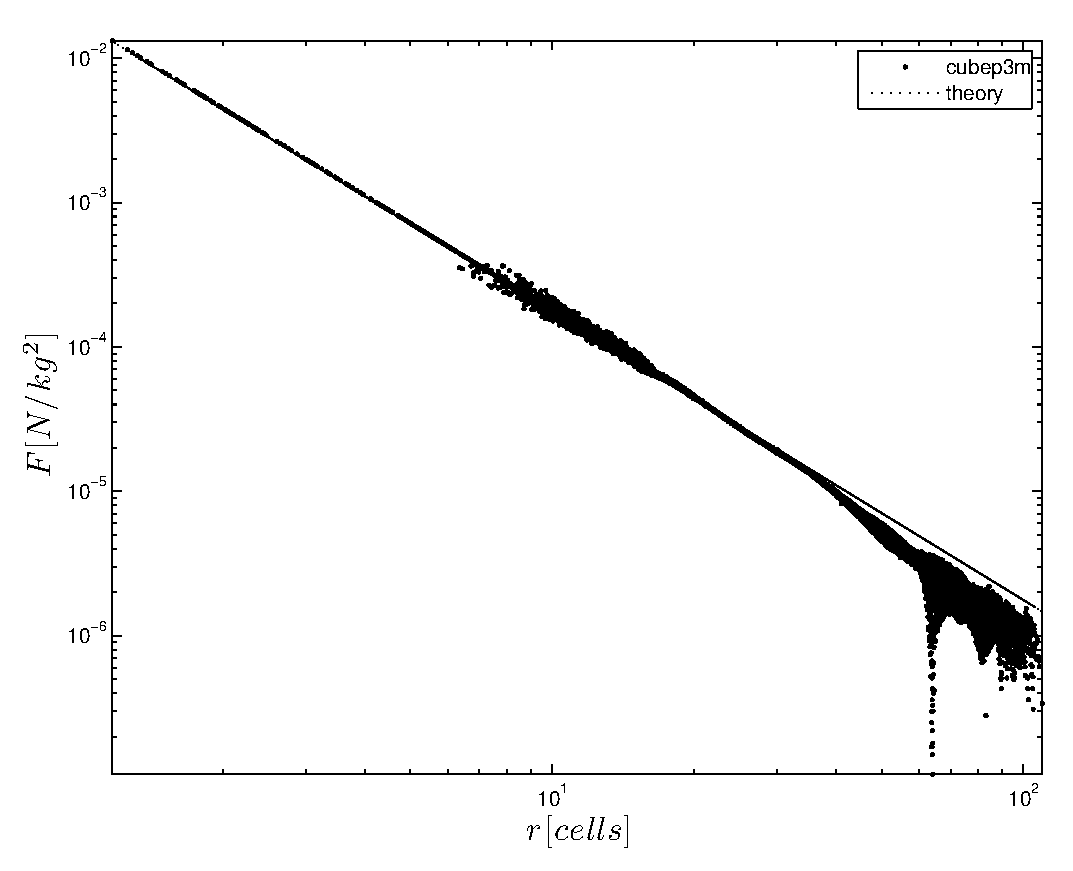
\includegraphics[width=3.2in]{graphs/densityForce_ppext=6.eps}
  \caption{Gravity force in the P$^3$M algorithm, compared with the exact $1/r^{2}$ law,
  in a CITA256 realization. The exact pp force has been extended to six fine mesh layers around each particle.
  Particles in the that range follow the exact curve, then we observe a much smaller scatter at 
  distance of the order of 6 fine grid, compared to Fig. \ref{fig:den_force_fracErr}. 
  The NGP interpolation scheme is again responsible for the scatter, but the effect is suppressed with increasing distances, and further suppressed by averaging over many time steps.. 
    \label{fig:den_force_ppext6}}
\end{center}
\end{figure}


 
\begin{figure}%[ht]
  \begin{center}
    \includegraphics[width=3.2in]{graphs/densityForce_fracErr_ppext=6.eps}
  \caption{Fractional error on the force in the P$^3$M algorithm, in the radial (top) and tangential (bottom) directions,
  in a CITA256 simulation in which the exact pp force extends to six fine mesh layers. 
  This was obtained over a single time step.
    \label{fig:den_force_fracErr_ppext6}}
\end{center}
\end{figure}

 
 
 To quantify the accuracy improvement versus computing time requirements, we performed the following test.
 We generate a set of initial conditions at a starting redshift of $z = 100$, with a box size equal to $ 200 h^{-1}\mbox{Mpc}$,
 and with $256^{3}$ particles. We evolve these CITA256 realizations with different ranges for the pp calculation, and compare 
 the resulting power spectra. For the results to be meaningful, we also need to use the same random seed for the random number generator,
 such that the only difference between different runs is the range of the pp force.
 Fig. \ref{fig:power} shows the dimensionless power spectrum of the different runs, where we see a significant gains in resolution
 when extending  PM to P$^{3}$M first, and when adding successive layers of fine cell mesh where the pp force is extended.
We have not plotted the results for higher numbers of layers, as the improvement becomes milder there: the fine grid calculations
are more accurate as the distance increases. For this reason, it seems that a range of a few layers, between 3 and 6, suffices 
to reduce most of the undesired NGP scatter.

Extending the pp calculation comes at a price, since the number of operation scales as  $N^{2}$ in the sub-domain. 
This cost is best capture by the increase of real time required by a fixed number of dedicated  {\small CPU}s 
to evolved the particles to the final redshift. Table \ref{table:cpu_pp_ext} presents this usage.

\begin{figure}
  \begin{center}
  \epsfig{file=graphs/pp_ext.eps,width=0.49\textwidth}
  \caption{ Dimensionless power spectrum for varying range of the exact pp force, compared to  {\small CAMB} \citep{Lewis:1999bs}.
  These CITA256 realizations evolved from a unique set of initial conditions at a starting redshift of $z = 100$, with a box size equal to $ 200 h^{-1}\mbox{Mpc}$ 
  until $z=0$. The only difference between the runs is the ranges of the pp calculation.}
    \label{fig:power}
  \end{center}
\end{figure}


\begin{table}
\begin{center}
\caption{Scaling in {\small CPU} resources as a function of the range of the pp interaction.
$N_{layers}$ refers to the number of fine mesh layers around a given cell, inside of which the force calculation
is purely given by the pp contribution. }
\begin{tabular}{|l|c|c|}
\hline 
             Type         & time (h)   \\
                  \hline
PM                         & 1.77 \\
P$^{3}$M             & 2.09 \\
\hline
$N_{layers}$       &          \\
\hline
 $1$ & 8.74 \\
 $2$ & 11.47\\
 $3$ & 14.30 \\
 $4$ & 18.87\\
 $5$ & 22.52\\
 $6$ & 29.62\\
 $7$ & 34.82\\
 $8$ & 47.00\\
 

\hline \hline
\end{tabular}
\label{table:cpu_pp_ext}
\end{center}
\end{table}

Perhaps the most relevant way to quantify the improvement of the calculation is to measure the impact on the halo mass function from these different CITA256 runs. Fig. \ref{fig:MassFunction_extpp} presents this comparison at redshift zero. About 11,000 haloes were found in the end, and we observe a good match with the Sheth-Tormen predictions. 

\begin{figure}
  \begin{center}
  \epsfig{file=graphs/MassFunction_pp_ranges.eps,width=0.49\textwidth}
  \caption{ Halo mass function for different ranges of the pp force calculation, compared to the predictions of Sheth-Tormen. {\bf (y-axis?)}}
    \label{fig:MassFunction_extpp}
  \end{center}
\end{figure}

